\section{Marco teórico específico}

Los sistemas distribuidos modernos rara vez utilizan un único modelo de RPC en todo su entorno; es habitual que un cliente consuma un servicio REST/JSON que internamente invoca un microservicio gRPC, el cual a su vez consulta datos expuestos vía JSON-RPC. Esta práctica construye un entorno reducido de esa arquitectura heterogénea: el cliente está escrito en Java; el procedimiento de cotización está implementado como un script bash que se ejecuta como CGI; y nginx funciona como el conmutador que conoce ambos extremos y media entre ellos, actuando simultáneamente como \emph{gateway} FastCGI y como \emph{reverse proxy} hacia un servicio JVM REST independiente.

\section{Arquitectura propuesta}

\begin{figure}[H]
\centering
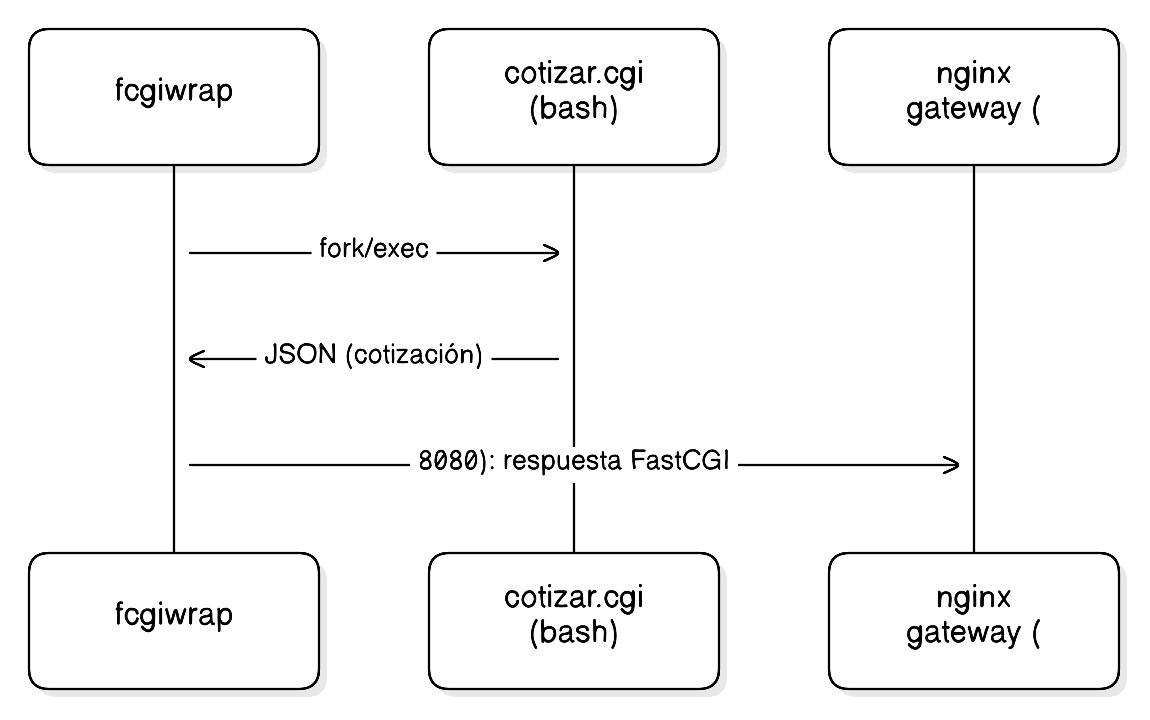
\includegraphics[width=0.85\linewidth]{../src/diagrams/practica3_secuencia.png}
\caption{Diagrama de secuencia de la práctica 3: RPC heterogéneo Java--nginx--CGI.}
\label{fig:p3-secuencia}
\end{figure}

\begin{figure}[H]
\centering
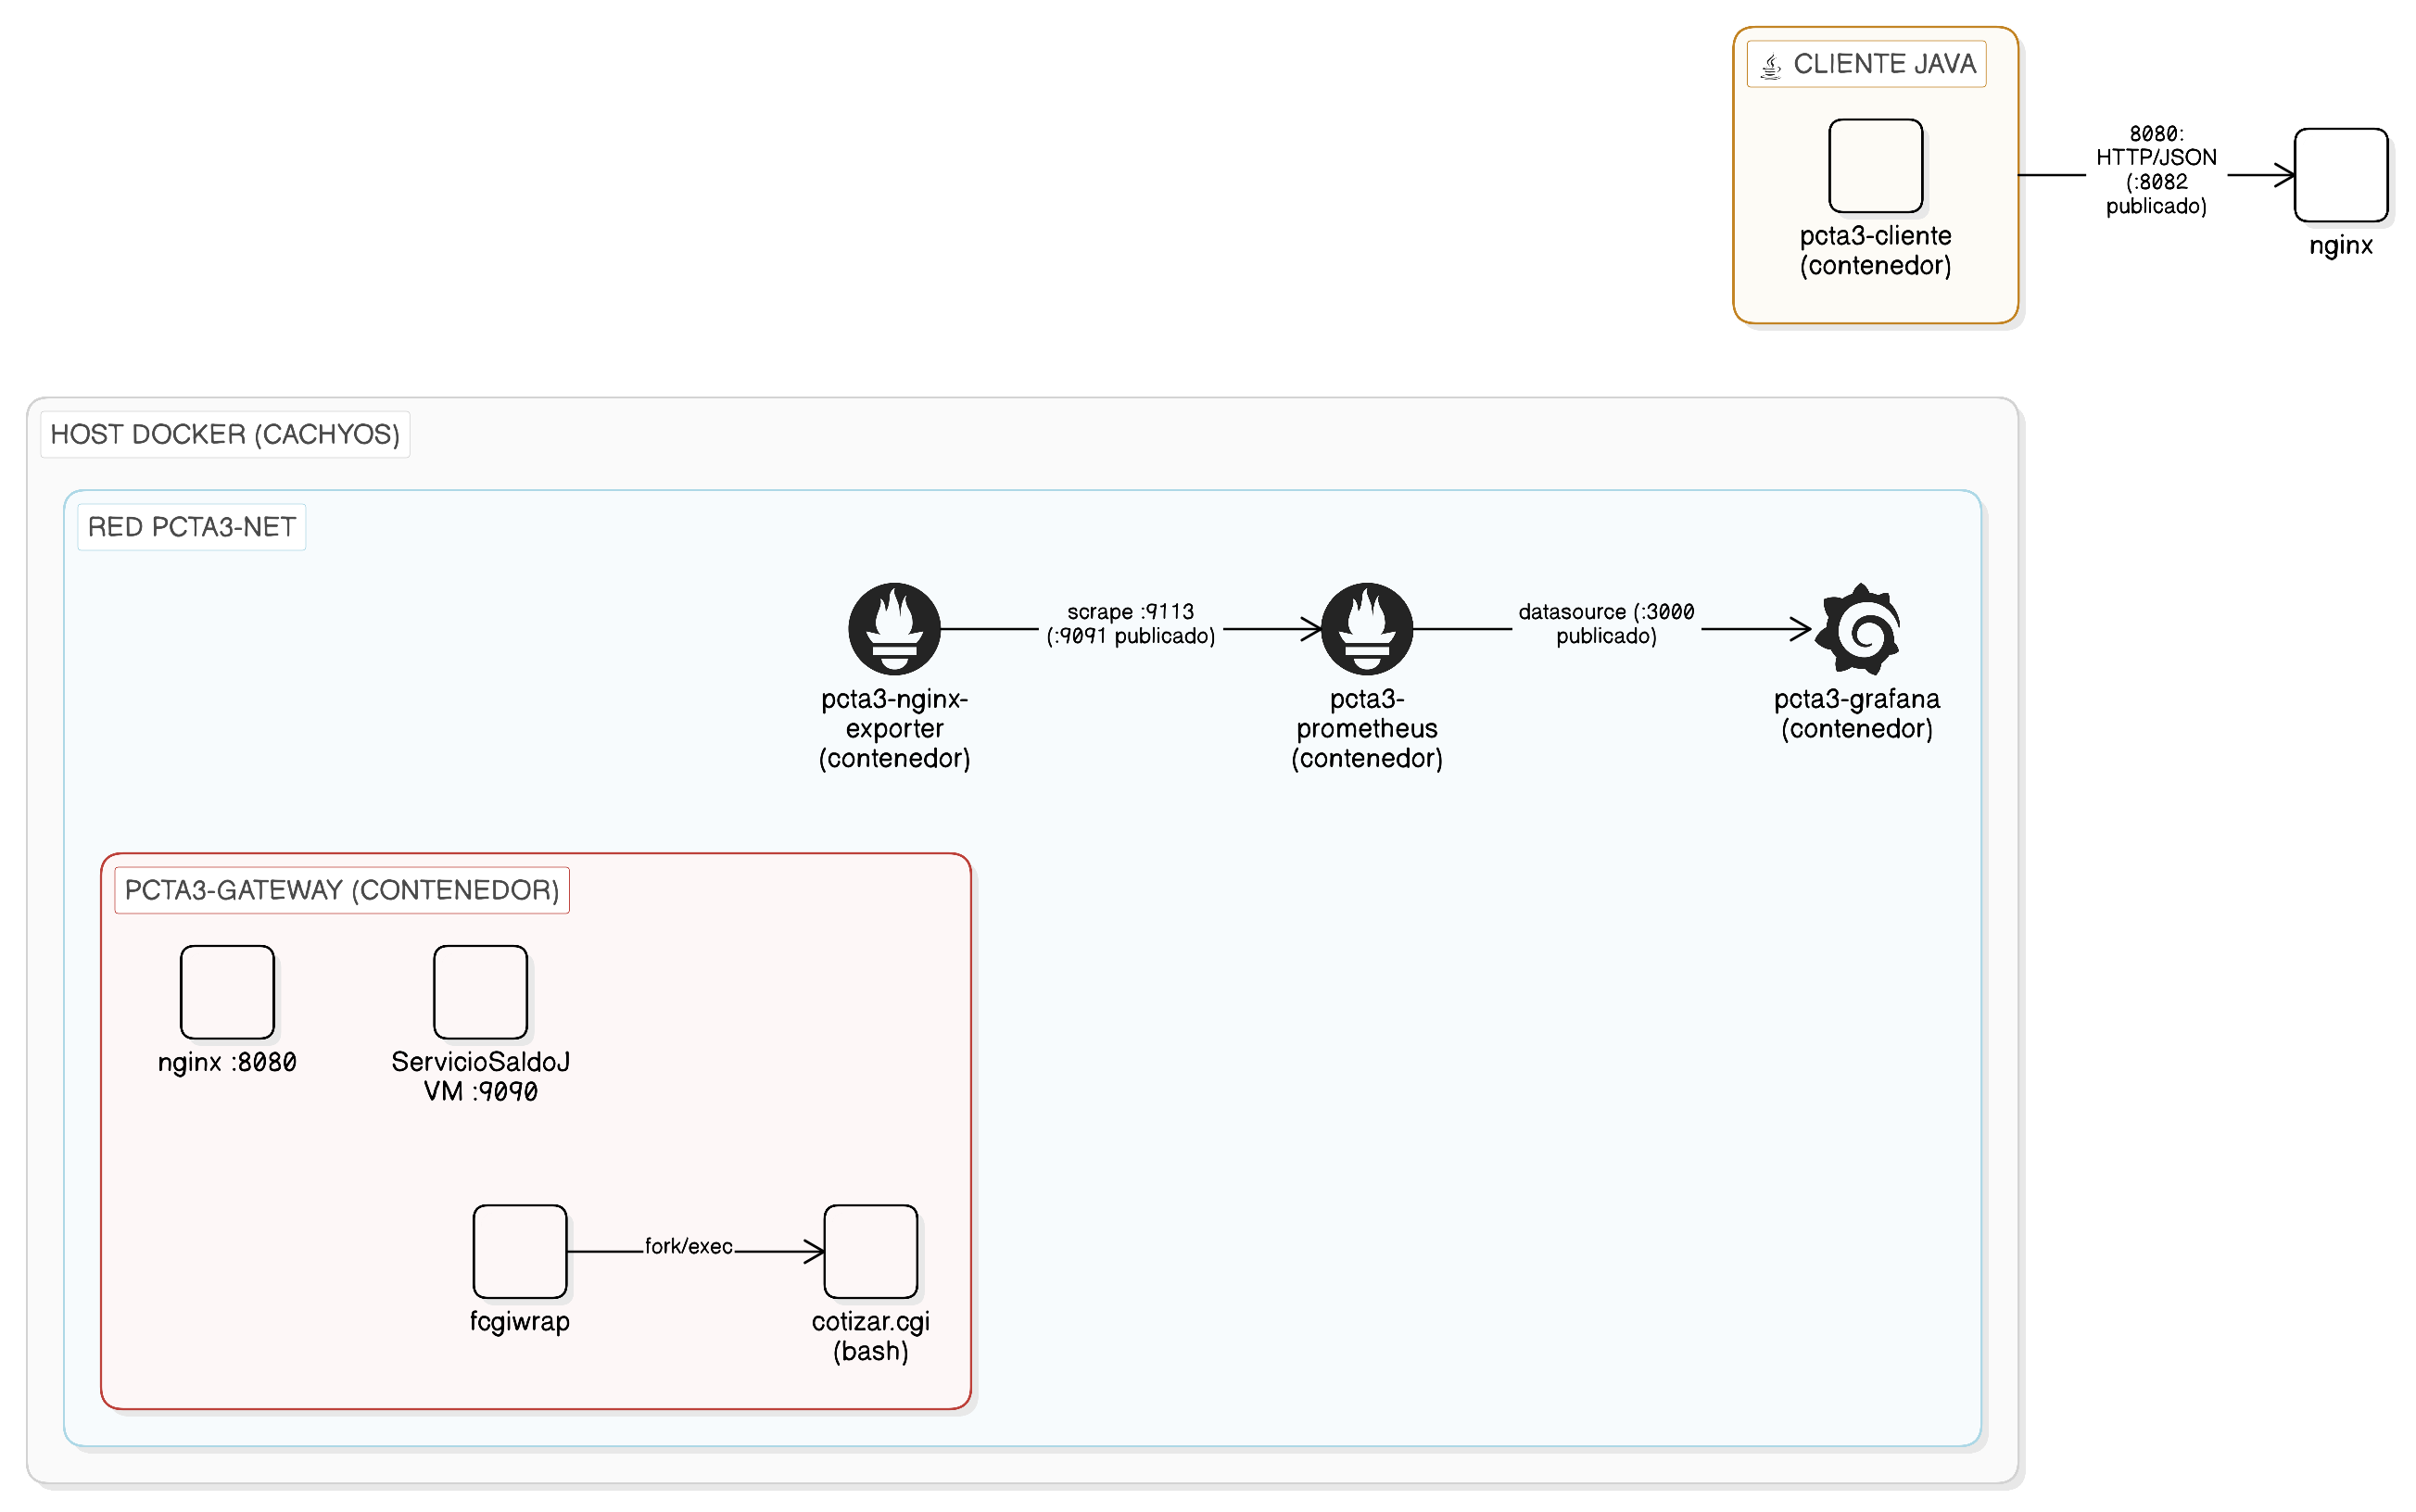
\includegraphics[width=\linewidth]{../src/diagrams/practica3_despliegue.png}
\caption{Diagrama de despliegue: contenedores, red interna \texttt{pcta3-net} y puertos publicados, incluido el stack de observabilidad del reto de extensión.}
\label{fig:p3-despliegue}
\end{figure}

A diferencia del diagrama de secuencia, que describe el orden temporal de una invocación, la Figura~\ref{fig:p3-despliegue} describe la topología física: qué proceso corre en qué contenedor, qué puertos cruzan la frontera del \emph{host} y cómo se conectan los nodos entre sí dentro de la red \texttt{pcta3-net}. El contenedor \texttt{pcta3-gateway} concentra tres roles (nginx, \texttt{fcgiwrap} y la JVM del servicio de saldo); los tres contenedores del stack de observabilidad (\texttt{nginx-exporter}, \texttt{prometheus}, \texttt{grafana}) se añadieron como parte del reto de extensión y se describen en la Sección~\ref{sec:p3-reto}.

\section{Entorno de trabajo}

Se construyó una única imagen Docker (\texttt{pcta3-heterogeneo}) que combina, sobre \texttt{fedora:36}, los tres papeles de la arquitectura: nginx como \emph{gateway}, \texttt{fcgiwrap} como puente FastCGI hacia el script CGI, y un JDK~17 para ejecutar el servicio JVM REST (\texttt{ServicioSaldoJVM}, escuchando en el puerto 9090 dentro del contenedor) que nginx expone bajo \texttt{/api/v1/saldo}. Un segundo contenedor (\texttt{pcta3-cliente}), basado en la misma imagen, ejecuta al cliente Java, conectado al primero mediante una red Docker dedicada (\texttt{pcta3-net}), reproduciendo la separación cliente/gateway sin necesidad de dos máquinas físicas.

\begin{lstlisting}[language=bash]
$ docker network create pcta3-net
$ docker run -d --name pcta3-gateway --network pcta3-net -p 8082:8080 pcta3-heterogeneo
$ docker run -d --name pcta3-cliente --network pcta3-net pcta3-heterogeneo sleep infinity
\end{lstlisting}

\begin{figure}[H]
\centering
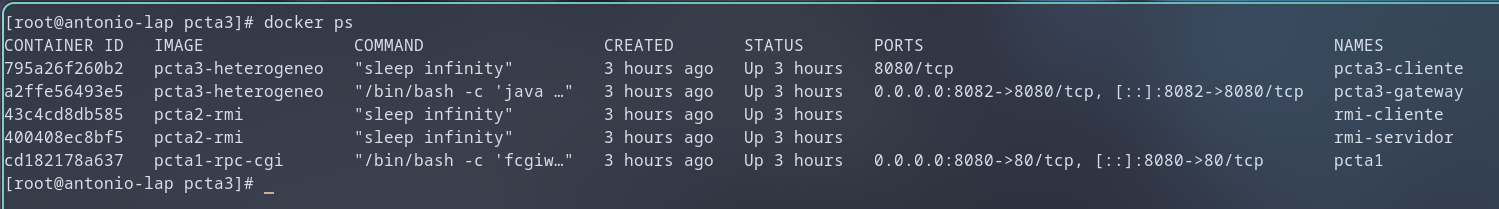
\includegraphics[width=\linewidth]{../src/ss/4.1.png}
\caption{Contenedores \texttt{pcta3-gateway} (puerto 8082 publicado) y \texttt{pcta3-cliente} en ejecución.}
\label{fig:p3-docker-ps}
\end{figure}

En la Figura~\ref{fig:p3-docker-ps}, el contenedor \texttt{pcta3-gateway} publica \texttt{8082->8080} hacia el anfitrión —la única puerta de entrada pública de toda la arquitectura— mientras que el servicio JVM del puerto 9090 no aparece en la columna \texttt{PORTS}: permanece privado dentro del contenedor, accesible únicamente a través del \emph{proxy} inverso de nginx. Esa asimetría es deliberada y refleja el papel de un \emph{gateway} en microservicios: los backends no se exponen directamente; el conmutador central es quien decide qué rutas existen hacia el exterior. La columna \texttt{COMMAND} del gateway muestra el arranque de la JVM junto con nginx y \texttt{fcgiwrap}, los tres procesos que en conjunto forman el \emph{runtime} heterogéneo de esta práctica.

\section{Servicio CGI/bash: cotizador de divisas}

Se implementó \texttt{/usr/lib/cgi-bin/rpc/cotizar.cgi}, que dada una divisa origen y un monto devuelve una cotización ficticia en pesos mexicanos, con una caché de idempotencia análoga a la del reto de la práctica 1 (cabecera \texttt{Idempotency-Key}).

\section{Servicio JVM REST --- \texttt{ServicioSaldoJVM.java}}

Se implementó un backend independiente con el \texttt{HttpServer} embebido del JDK (sin dependencias externas, dado que el contenedor no tiene salida a Internet para resolver un artefacto Maven):

\begin{lstlisting}[language=Java]
public class ServicioSaldoJVM {
    public static void main(String[] args) throws Exception {
        HttpServer server = HttpServer.create(new InetSocketAddress(9090), 0);
        server.createContext("/saldo", new SaldoHandler());
        server.start();
    }

    static class SaldoHandler implements HttpHandler {
        public void handle(HttpExchange exchange) throws IOException {
            String json = "{\"cuenta\":\"IPN-ESIMECU-0001\",\"saldo\":15340.75,\"moneda\":\"MXN\"}";
            byte[] bytes = json.getBytes(StandardCharsets.UTF_8);
            exchange.getResponseHeaders().add("Content-Type", "application/json; charset=UTF-8");
            exchange.sendResponseHeaders(200, bytes.length);
            exchange.getResponseBody().write(bytes);
            exchange.close();
        }
    }
}
\end{lstlisting}

\section{Configuración de nginx como gateway}

\begin{lstlisting}
upstream jvm_backend { server 127.0.0.1:9090; keepalive 16; }

server {
    listen 8080 default_server;
    server_name _;

    location /api/v1/cotizar {
        gzip off;
        root /usr/lib/cgi-bin;
        fastcgi_pass unix:/run/fcgiwrap.socket;
        include /etc/nginx/fastcgi_params;
        fastcgi_param SCRIPT_FILENAME /usr/lib/cgi-bin/rpc/cotizar.cgi;
        fastcgi_param DOCUMENT_ROOT   /usr/lib/cgi-bin/rpc;
        fastcgi_read_timeout 5s;
    }

    location /api/v1/saldo {
        proxy_pass          http://jvm_backend/saldo;
        proxy_read_timeout   5s;
        proxy_set_header     Host $host;
        proxy_set_header     X-Forwarded-For $remote_addr;
    }
}
\end{lstlisting}

\section{Cliente Java con \texttt{HttpClient}, reintentos y backoff}

\begin{lstlisting}[language=Java]
public static String cotizar(String host, String divisa, double monto) throws Exception {
    String idem = UUID.randomUUID().toString();
    String url  = String.format("http://%s:8080/api/v1/cotizar?divisa=%s&monto=%s",
                                 host, divisa, monto);
    HttpRequest req = HttpRequest.newBuilder(URI.create(url))
            .timeout(Duration.ofSeconds(3))
            .header("Accept", "application/json")
            .header("Idempotency-Key", idem)
            .GET().build();

    int intentos = 0; long espera = 250;
    while (true) {
        try {
            HttpResponse<String> r = HC.send(req, HttpResponse.BodyHandlers.ofString());
            if (r.statusCode() >= 500 && intentos < 3) throw new RuntimeException("5xx");
            return r.body();
        } catch (Exception e) {
            if (++intentos >= 4) throw e;
            Thread.sleep(espera); espera *= 2;
        }
    }
}
\end{lstlisting}

\begin{lstlisting}[language=bash]
$ docker exec pcta3-cliente java -cp /app/out mx.ipn.esimecu.rpc.ClienteIntegrador pcta3-gateway
{"divisa":"USD","monto":100.0,"tasa":17.25,"mxn":1725.0000,"fuente":"BANXICO-mock","servidor":"a2ffe56493e5"}
{"divisa":"EUR","monto":250.0,"tasa":18.40,"mxn":4600.0000,"fuente":"BANXICO-mock","servidor":"a2ffe56493e5"}
{"error":"divisa no soportada"}
{"cuenta":"IPN-ESIMECU-0001","saldo":15340.75,"moneda":"MXN"}
\end{lstlisting}

\begin{figure}[H]
\centering
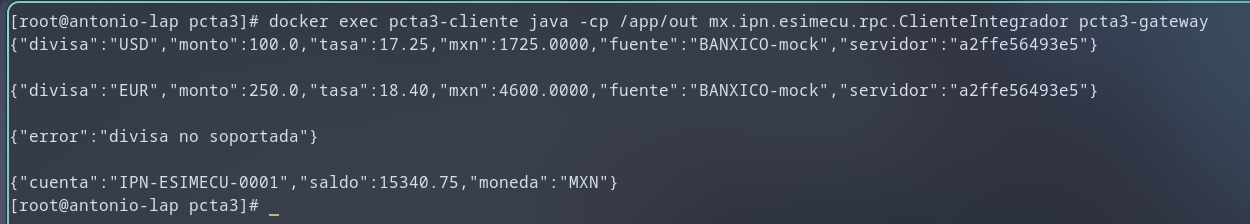
\includegraphics[width=\linewidth]{../src/ss/4.2.png}
\caption{Cliente Java invocando los dos ramos del gateway: cotizaciones (CGI/bash), divisa rechazada (422) y saldo (backend JVM).}
\label{fig:p3-cliente}
\end{figure}

Las cuatro respuestas de la Figura~\ref{fig:p3-cliente} evidencian la heterogeneidad que da nombre a la práctica. Las dos primeras (\texttt{USD}, \texttt{EUR}) fueron calculadas por un proceso bash lanzado por \texttt{fcgiwrap}; la tercera es el rechazo controlado de una divisa no soportada, propagado como código HTTP 422 y capturado por el cliente sin excepción; la cuarta proviene de un servidor Java persistente detrás del \emph{proxy} inverso. Para el cliente, las cuatro son indistinguibles: mismas URLs base, mismo formato JSON, misma llamada \texttt{HttpClient.send}. Esa uniformidad es el argumento central de la arquitectura: el \emph{gateway} absorbe la heterogeneidad de implementación (bash frente a JVM, FastCGI frente a HTTP \emph{proxied}) y ofrece al consumidor una interfaz homogénea, tal como los cinco componentes del modelo clásico prescriben que el stub oculte los detalles del transporte. El campo \texttt{servidor: a2ffe56493e5} en las cotizaciones —el \emph{hostname} del contenedor gateway— confirma dónde se ejecutó realmente el procedimiento.

\section{Diagnóstico con tcpdump y el log de acceso de nginx}

El log de acceso de nginx confirma que las cuatro peticiones anteriores llegaron efectivamente desde el cliente Java (encabezado \texttt{User-Agent: Java-http-client/17.0.7}), y distingue el código de estado de cada ramo:

\begin{lstlisting}
172.19.0.3 - - [.. ] "GET /api/v1/cotizar?divisa=USD&monto=100.0 HTTP/1.1" 200 121 "Java-http-client/17.0.7"
172.19.0.3 - - [.. ] "GET /api/v1/cotizar?divisa=EUR&monto=250.0 HTTP/1.1" 200 121 "Java-http-client/17.0.7"
172.19.0.3 - - [.. ] "GET /api/v1/cotizar?divisa=MXN&monto=10.0  HTTP/1.1" 422  43 "Java-http-client/17.0.7"
172.19.0.3 - - [.. ] "GET /api/v1/saldo                          HTTP/1.1" 200  61 "Java-http-client/17.0.7"
\end{lstlisting}

La captura de \texttt{tcpdump} sobre el puerto 8080 del contenedor \texttt{pcta3-gateway} corrobora la misma secuencia a nivel de segmentos TCP, mostrando las cuatro peticiones \texttt{GET} y sus respuestas \texttt{200}/\texttt{422} entre las direcciones internas de la red Docker (\texttt{172.19.0.3} cliente, \texttt{172.19.0.2} gateway):

\begin{lstlisting}
172.19.0.3.49966 > 172.19.0.2.8080: GET /api/v1/cotizar?divisa=USD&monto=100.0
172.19.0.2.8080 > 172.19.0.3.49966: HTTP/1.1 200 OK
172.19.0.3.49966 > 172.19.0.2.8080: GET /api/v1/cotizar?divisa=MXN&monto=10.0
172.19.0.2.8080 > 172.19.0.3.49966: HTTP/1.1 422 Unprocessable Entity
172.19.0.3.49966 > 172.19.0.2.8080: GET /api/v1/saldo
172.19.0.2.8080 > 172.19.0.3.49966: HTTP/1.1 200 OK
\end{lstlisting}

\begin{figure}[H]
\centering
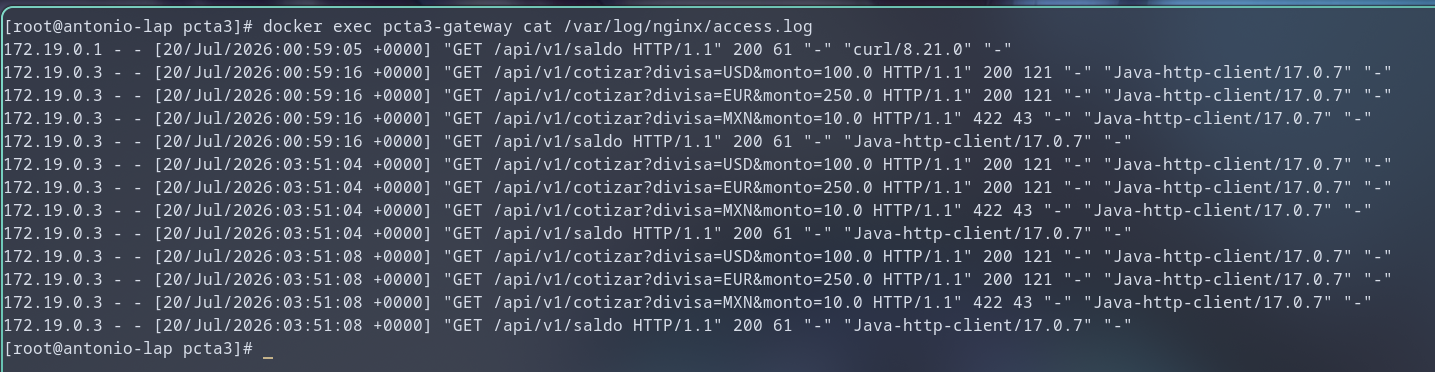
\includegraphics[width=\linewidth]{../src/ss/4.3.png}
\caption{Log de acceso de nginx en \texttt{pcta3-gateway}: cada invocación del cliente Java con su ruta, código de estado y \emph{User-Agent}.}
\label{fig:p3-diagnostico}
\end{figure}

El log de la Figura~\ref{fig:p3-diagnostico} es el punto de observabilidad natural del \emph{runtime}: por ser el conmutador por el que pasa todo el tráfico, nginx registra cada invocación con su origen, ruta, código de estado y tamaño de respuesta. Se distinguen la petición inicial de verificación hecha con \texttt{curl/8.21.0} desde el anfitrión (\texttt{172.19.0.1}) y las tandas posteriores del cliente Java (\texttt{Java-http-client/17.0.7} desde \texttt{172.19.0.3}), cada una con el patrón 200--200--422--200 que corresponde a las cuatro llamadas del programa. Este registro centralizado responde directamente a la pregunta de dónde instrumentar métricas en la arquitectura: una sola fuente captura la actividad de ambos ramos —CGI y JVM— sin tocar el código de ninguno de los dos backends.

\section{Comparación de latencia contra la práctica 2}
\label{sec:p3-latencia}

El entregable de esta práctica solicita comparar la latencia observada aquí contra la de la práctica 2 (Java RMI). Se midieron tres invocaciones equivalentes en esfuerzo de cómputo (una operación aritmética o una consulta trivial), excluyendo en los tres casos el costo de arranque de la JVM y de resolución de nombres, para aislar el costo específico de cada mecanismo de invocación:

\begin{itemize}
    \item \textbf{RMI nativo} (práctica 2): 50 invocaciones de \texttt{Calculadora.sumar()} sobre una conexión ya establecida (TLS incluido), medidas con \texttt{System.nanoTime()} alrededor de cada llamada.
    \item \textbf{HTTP hacia JVM persistente} (práctica 3, ramo \texttt{/api/v1/saldo}): 30 invocaciones con \texttt{curl -w \%\{time\_total\}}, atravesando nginx como \emph{reverse proxy} hacia el servicio JVM en el puerto 9090.
    \item \textbf{HTTP hacia CGI/bash} (práctica 3, ramo \texttt{/api/v1/cotizar}): 30 invocaciones con la misma técnica, atravesando nginx, \texttt{fcgiwrap} y un \texttt{fork}/\texttt{exec} de bash por petición.
\end{itemize}

\begin{table}[H]
\centering
\caption{Latencia de invocación remota por mecanismo (excluye arranque de JVM y resolución de nombres).}
\label{tab:latencia}
\begin{tabularx}{\linewidth}{lXccc}
\toprule
\textbf{Mecanismo} & \textbf{Ruta} & \textbf{Prom. (ms)} & \textbf{Mín. (ms)} & \textbf{Máx. (ms)} \\
\midrule
RMI nativo (TLS) & \texttt{Calculadora.sumar()} & 0.622 & 0.311 & 2.188 \\
HTTP / JVM persistente & \texttt{/api/v1/saldo} & 2.282 & 1.306 & 3.940 \\
HTTP / CGI (fork+exec) & \texttt{/api/v1/cotizar} & 18.060 & 14.790 & 21.859 \\
\bottomrule
\end{tabularx}
\end{table}

\begin{lstlisting}[language=bash]
$ docker exec rmi-cliente bash -c 'cd /rmi-lab/src && java $RMI_TLS_OPTS \
    mx.ipn.esimecu.rpc.LatencyBench rmi-servidor 50'
RMI sumar(): n=50 avg=0.622 ms min=0.311 ms max=2.188 ms

$ for i in $(seq 1 30); do curl -s -o /dev/null -w "%{time_total}\n" \
    'http://localhost:8082/api/v1/saldo'; done   # promedio: 2.282 ms

$ for i in $(seq 1 30); do curl -s -o /dev/null -w "%{time_total}\n" \
    'http://localhost:8082/api/v1/cotizar?divisa=USD&monto=1'; done   # promedio: 18.060 ms
\end{lstlisting}

\begin{figure}[H]
\centering
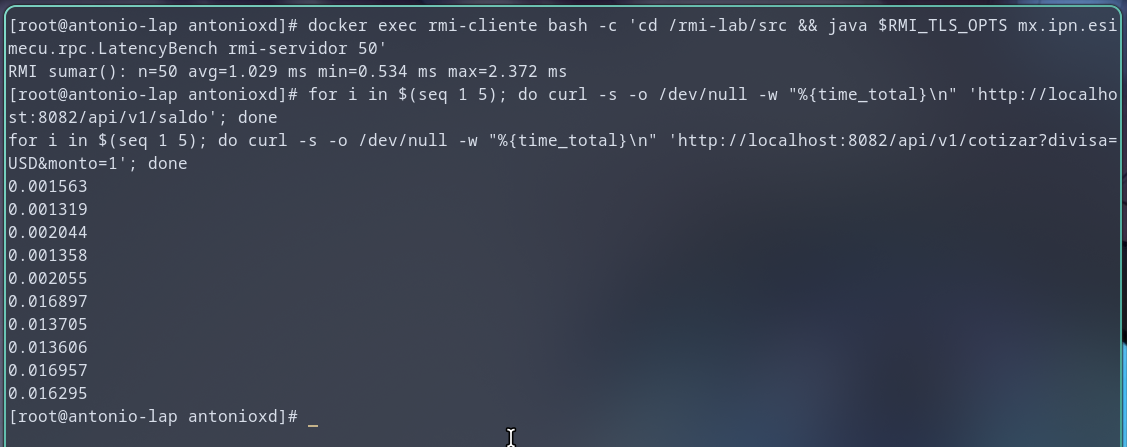
\includegraphics[width=0.9\linewidth]{../src/ss/p3-latencia.png}
\caption{Corrida confirmatoria: \texttt{LatencyBench} (RMI, $n=50$) y cinco muestras de \texttt{curl -w} para cada ruta de la práctica 3.}
\label{fig:p3-latencia}
\end{figure}

La Figura~\ref{fig:p3-latencia} es una segunda corrida, independiente de la usada para construir la Tabla~\ref{tab:latencia}, ejecutada minutos después; sus cinco muestras de \texttt{/api/v1/saldo} (1.3--2.1~ms) y de \texttt{/api/v1/cotizar} (13.6--17.0~ms) caen dentro del mismo orden de magnitud que los promedios de 30 muestras reportados en la tabla, y RMI repite un promedio submilisegundo (1.029~ms). La variación de un run a otro (por ejemplo, 0.622~ms vs.\ 1.029~ms en RMI) es esperable en un entorno de laboratorio compartido —contención de CPU con el resto de los contenedores activos, \emph{jitter} del planificador del anfitrión— y no cambia la conclusión: la brecha de aproximadamente un orden de magnitud entre CGI y las otras dos rutas se mantiene consistente entre ambas corridas.

Los resultados corroboran, con números reales, la respuesta teórica dada en el cuestionario de cierre de esta práctica sobre el costo de arranque de procesos: RMI —invocación directa sobre una conexión TCP persistente, sin intermediarios— resulta aproximadamente \textbf{3.7 veces más rápido} que atravesar nginx como \emph{proxy} hacia un servicio JVM igualmente persistente, y aproximadamente \textbf{29 veces más rápido} que invocar un script CGI que paga, en cada petición, el costo de que \texttt{fcgiwrap} haga \texttt{fork}/\texttt{exec} de un intérprete de bash nuevo. La diferencia entre las dos rutas de la práctica 3 (2.282~ms vs.\ 18.060~ms), a pesar de compartir el mismo \emph{gateway} nginx, aísla exactamente esa variable: el costo no está en el transporte HTTP ni en nginx, sino en el modelo de ejecución del backend. Esto confirma cuantitativamente por qué las arquitecturas de microservicios de alto volumen (Sección de casos de uso del marco teórico general) evitan CGI y prefieren procesos persistentes o RPC binario nativo como gRPC.

\section{Asociación con los cinco componentes RPC}

\begin{table}[H]
\centering
\caption{Asociación de la práctica 3 con la arquitectura clásica de RPC.}
\label{tab:componentes-rpc-p3}
\begin{tabularx}{\linewidth}{lX}
\toprule
\textbf{Componente RPC} & \textbf{Realización en la práctica 3} \\
\midrule
Cliente & \texttt{ClienteIntegrador.java} invocando un método Java que oculta la red. \\
Stub del cliente & \texttt{HttpRequest} + \texttt{HttpClient}: construyen la línea de petición, los encabezados y la URL. \\
RPC runtime & nginx (\emph{proxy} + FastCGI), \texttt{fcgiwrap} y la pila TCP/IP del sistema operativo. \\
Stub del servidor & Las primeras líneas de \texttt{cotizar.cgi}: parseo de variables CGI y validación de entradas. \\
Servidor & Cuerpo del script bash que calcula la cotización y la serializa como JSON (ramo CGI), o la clase \texttt{SaldoHandler} (ramo JVM). \\
\bottomrule
\end{tabularx}
\end{table}
